% Options for packages loaded elsewhere
\PassOptionsToPackage{unicode}{hyperref}
\PassOptionsToPackage{hyphens}{url}
\PassOptionsToPackage{dvipsnames,svgnames,x11names}{xcolor}
\documentclass[
]{article}
\usepackage{xcolor}
\usepackage[margin=1in]{geometry}
\usepackage{amsmath,amssymb}
\setcounter{secnumdepth}{-\maxdimen} % remove section numbering
\usepackage{iftex}
\ifPDFTeX
  \usepackage[T1]{fontenc}
  \usepackage[utf8]{inputenc}
  \usepackage{textcomp} % provide euro and other symbols
\else % if luatex or xetex
  \usepackage{unicode-math} % this also loads fontspec
  \defaultfontfeatures{Scale=MatchLowercase}
  \defaultfontfeatures[\rmfamily]{Ligatures=TeX,Scale=1}
\fi
\usepackage{lmodern}
\ifPDFTeX\else
  % xetex/luatex font selection
\fi
% Use upquote if available, for straight quotes in verbatim environments
\IfFileExists{upquote.sty}{\usepackage{upquote}}{}
\IfFileExists{microtype.sty}{% use microtype if available
  \usepackage[]{microtype}
  \UseMicrotypeSet[protrusion]{basicmath} % disable protrusion for tt fonts
}{}
\makeatletter
\@ifundefined{KOMAClassName}{% if non-KOMA class
  \IfFileExists{parskip.sty}{%
    \usepackage{parskip}
  }{% else
    \setlength{\parindent}{0pt}
    \setlength{\parskip}{6pt plus 2pt minus 1pt}}
}{% if KOMA class
  \KOMAoptions{parskip=half}}
\makeatother
\usepackage{color}
\usepackage{fancyvrb}
\newcommand{\VerbBar}{|}
\newcommand{\VERB}{\Verb[commandchars=\\\{\}]}
\DefineVerbatimEnvironment{Highlighting}{Verbatim}{commandchars=\\\{\}}
% Add ',fontsize=\small' for more characters per line
\usepackage{framed}
\definecolor{shadecolor}{RGB}{248,248,248}
\newenvironment{Shaded}{\begin{snugshade}}{\end{snugshade}}
\newcommand{\AlertTok}[1]{\textcolor[rgb]{0.94,0.16,0.16}{#1}}
\newcommand{\AnnotationTok}[1]{\textcolor[rgb]{0.56,0.35,0.01}{\textbf{\textit{#1}}}}
\newcommand{\AttributeTok}[1]{\textcolor[rgb]{0.13,0.29,0.53}{#1}}
\newcommand{\BaseNTok}[1]{\textcolor[rgb]{0.00,0.00,0.81}{#1}}
\newcommand{\BuiltInTok}[1]{#1}
\newcommand{\CharTok}[1]{\textcolor[rgb]{0.31,0.60,0.02}{#1}}
\newcommand{\CommentTok}[1]{\textcolor[rgb]{0.56,0.35,0.01}{\textit{#1}}}
\newcommand{\CommentVarTok}[1]{\textcolor[rgb]{0.56,0.35,0.01}{\textbf{\textit{#1}}}}
\newcommand{\ConstantTok}[1]{\textcolor[rgb]{0.56,0.35,0.01}{#1}}
\newcommand{\ControlFlowTok}[1]{\textcolor[rgb]{0.13,0.29,0.53}{\textbf{#1}}}
\newcommand{\DataTypeTok}[1]{\textcolor[rgb]{0.13,0.29,0.53}{#1}}
\newcommand{\DecValTok}[1]{\textcolor[rgb]{0.00,0.00,0.81}{#1}}
\newcommand{\DocumentationTok}[1]{\textcolor[rgb]{0.56,0.35,0.01}{\textbf{\textit{#1}}}}
\newcommand{\ErrorTok}[1]{\textcolor[rgb]{0.64,0.00,0.00}{\textbf{#1}}}
\newcommand{\ExtensionTok}[1]{#1}
\newcommand{\FloatTok}[1]{\textcolor[rgb]{0.00,0.00,0.81}{#1}}
\newcommand{\FunctionTok}[1]{\textcolor[rgb]{0.13,0.29,0.53}{\textbf{#1}}}
\newcommand{\ImportTok}[1]{#1}
\newcommand{\InformationTok}[1]{\textcolor[rgb]{0.56,0.35,0.01}{\textbf{\textit{#1}}}}
\newcommand{\KeywordTok}[1]{\textcolor[rgb]{0.13,0.29,0.53}{\textbf{#1}}}
\newcommand{\NormalTok}[1]{#1}
\newcommand{\OperatorTok}[1]{\textcolor[rgb]{0.81,0.36,0.00}{\textbf{#1}}}
\newcommand{\OtherTok}[1]{\textcolor[rgb]{0.56,0.35,0.01}{#1}}
\newcommand{\PreprocessorTok}[1]{\textcolor[rgb]{0.56,0.35,0.01}{\textit{#1}}}
\newcommand{\RegionMarkerTok}[1]{#1}
\newcommand{\SpecialCharTok}[1]{\textcolor[rgb]{0.81,0.36,0.00}{\textbf{#1}}}
\newcommand{\SpecialStringTok}[1]{\textcolor[rgb]{0.31,0.60,0.02}{#1}}
\newcommand{\StringTok}[1]{\textcolor[rgb]{0.31,0.60,0.02}{#1}}
\newcommand{\VariableTok}[1]{\textcolor[rgb]{0.00,0.00,0.00}{#1}}
\newcommand{\VerbatimStringTok}[1]{\textcolor[rgb]{0.31,0.60,0.02}{#1}}
\newcommand{\WarningTok}[1]{\textcolor[rgb]{0.56,0.35,0.01}{\textbf{\textit{#1}}}}
\usepackage{longtable,booktabs,array}
\usepackage{calc} % for calculating minipage widths
% Correct order of tables after \paragraph or \subparagraph
\usepackage{etoolbox}
\makeatletter
\patchcmd\longtable{\par}{\if@noskipsec\mbox{}\fi\par}{}{}
\makeatother
% Allow footnotes in longtable head/foot
\IfFileExists{footnotehyper.sty}{\usepackage{footnotehyper}}{\usepackage{footnote}}
\makesavenoteenv{longtable}
\usepackage{graphicx}
\makeatletter
\newsavebox\pandoc@box
\newcommand*\pandocbounded[1]{% scales image to fit in text height/width
  \sbox\pandoc@box{#1}%
  \Gscale@div\@tempa{\textheight}{\dimexpr\ht\pandoc@box+\dp\pandoc@box\relax}%
  \Gscale@div\@tempb{\linewidth}{\wd\pandoc@box}%
  \ifdim\@tempb\p@<\@tempa\p@\let\@tempa\@tempb\fi% select the smaller of both
  \ifdim\@tempa\p@<\p@\scalebox{\@tempa}{\usebox\pandoc@box}%
  \else\usebox{\pandoc@box}%
  \fi%
}
% Set default figure placement to htbp
\def\fps@figure{htbp}
\makeatother
\setlength{\emergencystretch}{3em} % prevent overfull lines
\providecommand{\tightlist}{%
  \setlength{\itemsep}{0pt}\setlength{\parskip}{0pt}}
\usepackage{bookmark}
\IfFileExists{xurl.sty}{\usepackage{xurl}}{} % add URL line breaks if available
\urlstyle{same}
\hypersetup{
  pdftitle={Socioeconomic Determinants of 2020 U.S. Presidential Election County-Level Voter Turnout},
  pdfauthor={Yuen Ler Chow, John Rho, and Henry Wu},
  colorlinks=true,
  linkcolor={Maroon},
  filecolor={Maroon},
  citecolor={Blue},
  urlcolor={blue},
  pdfcreator={LaTeX via pandoc}}

\title{Socioeconomic Determinants of 2020 U.S. Presidential Election
County-Level Voter Turnout}
\usepackage{etoolbox}
\makeatletter
\providecommand{\subtitle}[1]{% add subtitle to \maketitle
  \apptocmd{\@title}{\par {\large #1 \par}}{}{}
}
\makeatother
\subtitle{Exploratory Data Analysis}
\author{Yuen Ler Chow, John Rho, and Henry Wu}
\date{}

\begin{document}
\maketitle

\section{Data Description}\label{data-description}

There are a few different data sources joined together to make this
dataset. The turnout rate data is calculating by dividing the voter
turnout for the 2020 presidential election in each county (from the
\href{https://doi.org/10.7910/DVN/VOQCHQ}{MIT Election Lab}) by the
voting-eligible population (U.S. citizens age 18 and up) according to
the
\href{https://data.census.gov/table/ACSDT5Y2020.B05003?t=Citizenship&g=010XX00US$0500000&y=2020&d=ACS\%205-Year\%20Estimates\%20Detailed\%20Tables&moe=false&tp=true}{2020
5-year American Community Survey} released by the U.S. Census Bureau.
The resulting turnout rate should be a proportion between 0 and 1. The
exception for the voter turnout data is Alaska, whose voter turnout data
is organized by election districts instead of borough and Census areas
(Alaska's county equivalents). To have this data be consistent with the
predictor variables, I got estimates for Alaska voter turnout data by
borough and Census area from a
\href{https://rrhelections.com/index.php/2021/04/13/alaska-presidential-results-by-county-equivalent-1960-2020/9/}{blog
post}.

The
\href{https://opportunityinsights.org/wp-content/uploads/2024/07/Table_8_county_covariates.csv}{predictors}
(county-level demographic and socioeconomic characteristics) are from
Opportunity Insights, a Harvard-based research lab studying economic
opportunity in the United States. Descriptions of the variables can be
found
\href{https://opportunityinsights.org/wp-content/uploads/2019/07/Codebook-for-Table-10.pdf}{here}.
Datasets for FIPS
\href{https://www2.census.gov/geo/docs/reference/codes2020/national_state2020.txt}{state}
and
\href{https://www2.census.gov/geo/docs/reference/codes2020/national_county2020.txt}{county}
codes are also used to merge the data sources.

\section{Setup}\label{setup}

\begin{Shaded}
\begin{Highlighting}[]
\FunctionTok{rm}\NormalTok{(}\AttributeTok{list =} \FunctionTok{ls}\NormalTok{())}
\FunctionTok{require}\NormalTok{(readr)}
\FunctionTok{require}\NormalTok{(tidyr)}
\FunctionTok{require}\NormalTok{(dplyr)}
\FunctionTok{require}\NormalTok{(knitr)}
\FunctionTok{require}\NormalTok{(glmnet)}
\FunctionTok{require}\NormalTok{(pheatmap)}
\end{Highlighting}
\end{Shaded}

\begin{Shaded}
\begin{Highlighting}[]
\NormalTok{turnout\_data }\OtherTok{\textless{}{-}} \FunctionTok{read.csv}\NormalTok{(}\StringTok{"../data/processed/data.csv"}\NormalTok{)}
\FunctionTok{head}\NormalTok{(turnout\_data)}
\end{Highlighting}
\end{Shaded}

\begin{verbatim}
##     State         County fips frac_coll_plus2010 foreign_share2010
## 1 Alabama Autauga County 1001         0.22199036       0.020154603
## 2 Alabama Baldwin County 1003         0.26071036       0.037591625
## 3 Alabama Barbour County 1005         0.13349621       0.028143950
## 4 Alabama    Bibb County 1007         0.09924053       0.006859188
## 5 Alabama  Blount County 1009         0.12633450       0.047343444
## 6 Alabama Bullock County 1011         0.10972187       0.013493270
##   med_hhinc2016 poor_share2010 share_white2010 share_black2010 share_hisp2010
## 1      54052.80      0.1059177       0.7724616      0.18134174     0.02400542
## 2      52003.09      0.1229422       0.8350479      0.09752284     0.04384824
## 3      33114.85      0.2506308       0.4675311      0.47190151     0.05051535
## 4      39846.45      0.1268499       0.7502073      0.22282349     0.01771765
## 5      46361.12      0.1331379       0.8888734      0.01500297     0.08070200
## 6      31304.78      0.2804486       0.2191680      0.70221734     0.07119296
##   share_asian2010 gsmn_math_g3_2013 rent_twobed2015 singleparent_share2010
## 1    0.0078302799          2.759864        739.3654              0.2833759
## 2    0.0059535136          2.792510        816.8452              0.2778664
## 3    0.0036882064          1.600009        527.2908              0.4680706
## 4    0.0007418721          1.531674        604.2776              0.3201363
## 5    0.0018735955          2.815403        567.6959              0.2589052
## 6    0.0017932489          1.039439        266.0000              0.5778636
##   traveltime15_2010   emp2000 ln_wage_growth_hs_grad popdensity2010
## 1         0.2041625 0.6095865            -0.06331379       91.80268
## 2         0.2753262 0.5770263             0.03009291      114.64751
## 3         0.3760492 0.4532710             0.18936642       31.02921
## 4         0.2526830 0.4942406            -0.02007263       36.80634
## 5         0.1943438 0.5778096             0.09646260       88.90219
## 6         0.3921350 0.3746639             0.36383346       17.52395
##   ann_avg_job_growth_2004_2013 job_density_2013 turnout.rate
## 1                  0.010145103        40.719135    0.6618366
## 2                  0.012950056        50.085987    0.6529056
## 3                 -0.020755908         9.230672    0.5402712
## 4                 -0.004644653        12.875392    0.5456975
## 5                 -0.008120399        36.175354    0.6419098
## 6                  0.026254078         6.954023    0.5908043
\end{verbatim}

\section{Descriptive Statistics}\label{descriptive-statistics}

We have no categorical variables. For each of our continuous variables,
we summarize the number of missing values, the mean, median, standard
deviation, interquartile range, minimum value, and maximum value.

\begin{Shaded}
\begin{Highlighting}[]
\NormalTok{predictors }\OtherTok{\textless{}{-}} \FunctionTok{names}\NormalTok{(turnout\_data)[}\SpecialCharTok{!}\NormalTok{(}\FunctionTok{names}\NormalTok{(turnout\_data) }\SpecialCharTok{\%in\%} \FunctionTok{c}\NormalTok{(}\StringTok{\textquotesingle{}State\textquotesingle{}}\NormalTok{, }\StringTok{\textquotesingle{}County\textquotesingle{}}\NormalTok{, }\StringTok{\textquotesingle{}fips\textquotesingle{}}\NormalTok{))]}
\NormalTok{summary\_table }\OtherTok{\textless{}{-}} \FunctionTok{data.frame}\NormalTok{()}

\ControlFlowTok{for}\NormalTok{ (predictor }\ControlFlowTok{in}\NormalTok{ predictors) \{}
\NormalTok{  column }\OtherTok{\textless{}{-}}\NormalTok{ turnout\_data[[predictor]]}
\NormalTok{  num\_missing }\OtherTok{\textless{}{-}} \FunctionTok{sum}\NormalTok{(}\FunctionTok{is.na}\NormalTok{(column))}
\NormalTok{  mean\_var }\OtherTok{\textless{}{-}} \FunctionTok{mean}\NormalTok{(column, }\AttributeTok{na.rm =} \ConstantTok{TRUE}\NormalTok{)}
\NormalTok{  median\_var }\OtherTok{\textless{}{-}} \FunctionTok{median}\NormalTok{(column, }\AttributeTok{na.rm =} \ConstantTok{TRUE}\NormalTok{)}
\NormalTok{  sd\_var }\OtherTok{\textless{}{-}} \FunctionTok{sd}\NormalTok{(column, }\AttributeTok{na.rm =} \ConstantTok{TRUE}\NormalTok{)}
\NormalTok{  iqr\_var }\OtherTok{\textless{}{-}} \FunctionTok{IQR}\NormalTok{(column, }\AttributeTok{na.rm =} \ConstantTok{TRUE}\NormalTok{)}
\NormalTok{  min\_var }\OtherTok{\textless{}{-}} \FunctionTok{min}\NormalTok{(column, }\AttributeTok{na.rm =} \ConstantTok{TRUE}\NormalTok{)}
\NormalTok{  max\_var }\OtherTok{\textless{}{-}} \FunctionTok{max}\NormalTok{(column, }\AttributeTok{na.rm =} \ConstantTok{TRUE}\NormalTok{)}

\NormalTok{  summary\_table }\OtherTok{\textless{}{-}} \FunctionTok{rbind}\NormalTok{(summary\_table, }\FunctionTok{data.frame}\NormalTok{(}
    \AttributeTok{Variable =}\NormalTok{ predictor,}
    \AttributeTok{Missing =}\NormalTok{ num\_missing,}
    \AttributeTok{Mean =} \FunctionTok{round}\NormalTok{(mean\_var, }\DecValTok{2}\NormalTok{),}
    \AttributeTok{Median =} \FunctionTok{round}\NormalTok{(median\_var, }\DecValTok{2}\NormalTok{),}
    \AttributeTok{SD =} \FunctionTok{round}\NormalTok{(sd\_var, }\DecValTok{2}\NormalTok{),}
    \AttributeTok{IQR =} \FunctionTok{round}\NormalTok{(iqr\_var, }\DecValTok{2}\NormalTok{),}
    \AttributeTok{Min =} \FunctionTok{round}\NormalTok{(min\_var, }\DecValTok{2}\NormalTok{),}
    \AttributeTok{Max =} \FunctionTok{round}\NormalTok{(max\_var, }\DecValTok{2}\NormalTok{)}
\NormalTok{  ))}
\NormalTok{\}}

\FunctionTok{kable}\NormalTok{(summary\_table)}
\end{Highlighting}
\end{Shaded}

\begin{longtable}[]{@{}
  >{\raggedright\arraybackslash}p{(\linewidth - 14\tabcolsep) * \real{0.3152}}
  >{\raggedleft\arraybackslash}p{(\linewidth - 14\tabcolsep) * \real{0.0870}}
  >{\raggedleft\arraybackslash}p{(\linewidth - 14\tabcolsep) * \real{0.0978}}
  >{\raggedleft\arraybackslash}p{(\linewidth - 14\tabcolsep) * \real{0.0978}}
  >{\raggedleft\arraybackslash}p{(\linewidth - 14\tabcolsep) * \real{0.0978}}
  >{\raggedleft\arraybackslash}p{(\linewidth - 14\tabcolsep) * \real{0.0978}}
  >{\raggedleft\arraybackslash}p{(\linewidth - 14\tabcolsep) * \real{0.0978}}
  >{\raggedleft\arraybackslash}p{(\linewidth - 14\tabcolsep) * \real{0.1087}}@{}}
\toprule\noalign{}
\begin{minipage}[b]{\linewidth}\raggedright
Variable
\end{minipage} & \begin{minipage}[b]{\linewidth}\raggedleft
Missing
\end{minipage} & \begin{minipage}[b]{\linewidth}\raggedleft
Mean
\end{minipage} & \begin{minipage}[b]{\linewidth}\raggedleft
Median
\end{minipage} & \begin{minipage}[b]{\linewidth}\raggedleft
SD
\end{minipage} & \begin{minipage}[b]{\linewidth}\raggedleft
IQR
\end{minipage} & \begin{minipage}[b]{\linewidth}\raggedleft
Min
\end{minipage} & \begin{minipage}[b]{\linewidth}\raggedleft
Max
\end{minipage} \\
\midrule\noalign{}
\endhead
\bottomrule\noalign{}
\endlastfoot
frac\_coll\_plus2010 & 0 & 0.19 & 0.17 & 0.09 & 0.09 & 0.04 & 0.71 \\
foreign\_share2010 & 0 & 0.04 & 0.02 & 0.06 & 0.04 & 0.00 & 0.72 \\
med\_hhinc2016 & 1 & 48980.92 & 47127.10 & 13398.03 & 14687.30 &
20170.89 & 129150.34 \\
poor\_share2010 & 0 & 0.16 & 0.15 & 0.06 & 0.08 & 0.00 & 0.53 \\
share\_white2010 & 0 & 0.78 & 0.86 & 0.20 & 0.27 & 0.03 & 0.99 \\
share\_black2010 & 0 & 0.09 & 0.02 & 0.15 & 0.10 & 0.00 & 0.86 \\
share\_hisp2010 & 0 & 0.08 & 0.03 & 0.13 & 0.07 & 0.00 & 0.96 \\
share\_asian2010 & 21 & 0.01 & 0.00 & 0.02 & 0.01 & 0.00 & 0.43 \\
gsmn\_math\_g3\_2013 & 73 & 3.21 & 3.24 & 0.78 & 0.98 & -0.66 & 6.58 \\
rent\_twobed2015 & 76 & 692.34 & 642.51 & 205.04 & 195.93 & 236.00 &
2085.23 \\
singleparent\_share2010 & 0 & 0.31 & 0.30 & 0.09 & 0.10 & 0.00 & 0.81 \\
traveltime15\_2010 & 0 & 0.40 & 0.38 & 0.14 & 0.19 & 0.10 & 0.99 \\
emp2000 & 0 & 0.57 & 0.58 & 0.08 & 0.10 & 0.24 & 0.84 \\
ln\_wage\_growth\_hs\_grad & 684 & 0.08 & 0.07 & 0.14 & 0.13 & -0.72 &
0.91 \\
popdensity2010 & 1 & 262.67 & 45.30 & 1774.99 & 96.74 & 0.04 &
70583.63 \\
ann\_avg\_job\_growth\_2004\_2013 & 5 & 0.00 & 0.00 & 0.01 & 0.02 &
-0.08 & 0.12 \\
job\_density\_2013 & 2 & 124.24 & 18.47 & 862.85 & 43.30 & 0.02 &
36663.16 \\
turnout.rate & 0 & 0.66 & 0.66 & 0.11 & 0.14 & 0.19 & 1.58 \\
\end{longtable}

\begin{Shaded}
\begin{Highlighting}[]
\FunctionTok{dim}\NormalTok{(turnout\_data)}
\end{Highlighting}
\end{Shaded}

\begin{verbatim}
## [1] 3141   21
\end{verbatim}

\subsection{Missingness}\label{missingness}

Most variables have either zero or a small fraction of observations
missing. The exception is \texttt{ln\_wage\_growth\_hs\_grad}, which has
21.8\% of its observations missing. To handle the missing data, we drop
the \texttt{ln\_wage\_growth\_hs\_grad} variable altogether and drop the
counties that have missing data in at least one of the remaining
variables.

\begin{Shaded}
\begin{Highlighting}[]
\NormalTok{turnout\_data }\OtherTok{\textless{}{-}} \FunctionTok{select}\NormalTok{(turnout\_data, }\SpecialCharTok{{-}}\NormalTok{ln\_wage\_growth\_hs\_grad)}
\NormalTok{turnout\_data }\OtherTok{\textless{}{-}} \FunctionTok{subset}\NormalTok{(turnout\_data, }\FunctionTok{apply}\NormalTok{(turnout\_data, }\DecValTok{1}\NormalTok{, }\AttributeTok{FUN =} \ControlFlowTok{function}\NormalTok{(x) \{}\SpecialCharTok{!}\FunctionTok{any}\NormalTok{(}\FunctionTok{is.na}\NormalTok{(x))\}))}
\FunctionTok{dim}\NormalTok{(turnout\_data)}
\end{Highlighting}
\end{Shaded}

\begin{verbatim}
## [1] 2999   20
\end{verbatim}

\section{Exploratory Graphs}\label{exploratory-graphs}

\subsection{Turnout Rate}\label{turnout-rate}

There is one invalid value for turnout rate greater than 1, so we set it
equal to 1. The histogram shows that the turnout rates are approximately
normally distributed.

\begin{Shaded}
\begin{Highlighting}[]
\FunctionTok{subset}\NormalTok{(turnout\_data, turnout.rate }\SpecialCharTok{\textgreater{}} \DecValTok{1}\NormalTok{)[}\FunctionTok{c}\NormalTok{(}\StringTok{\textquotesingle{}State\textquotesingle{}}\NormalTok{, }\StringTok{\textquotesingle{}County\textquotesingle{}}\NormalTok{, }\StringTok{\textquotesingle{}turnout.rate\textquotesingle{}}\NormalTok{)]}
\end{Highlighting}
\end{Shaded}

\begin{verbatim}
##             State        County turnout.rate
## 2391 South Dakota Hanson County     1.006321
\end{verbatim}

\begin{Shaded}
\begin{Highlighting}[]
\NormalTok{turnout\_data }\OtherTok{\textless{}{-}}\NormalTok{ turnout\_data }\SpecialCharTok{\%\textgreater{}\%}
  \FunctionTok{mutate}\NormalTok{(}\AttributeTok{turnout.rate =} \FunctionTok{case\_when}\NormalTok{(}
\NormalTok{    turnout.rate }\SpecialCharTok{\textgreater{}} \DecValTok{1} \SpecialCharTok{\textasciitilde{}} \DecValTok{1}\NormalTok{,}
    \AttributeTok{.default =}\NormalTok{ turnout.rate}
\NormalTok{  ))}
\FunctionTok{hist}\NormalTok{(turnout\_data}\SpecialCharTok{$}\NormalTok{turnout.rate, }\AttributeTok{main =} \StringTok{\textquotesingle{}Histogram of Turnout Rate\textquotesingle{}}\NormalTok{, }\AttributeTok{xlab =} \StringTok{\textquotesingle{}Turnout Rate\textquotesingle{}}\NormalTok{)}
\end{Highlighting}
\end{Shaded}

\pandocbounded{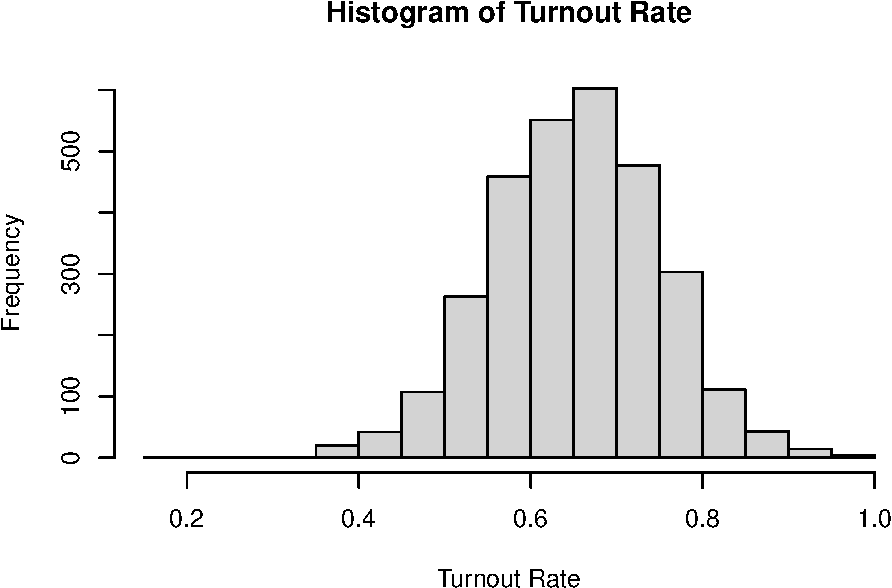
\includegraphics[keepaspectratio]{finalPaper_files/figure-latex/turnout-1.pdf}}

\subsection{Math Scores}\label{math-scores}

There are a few invalid values for mean math scores less than 0, so we
set them equal to 0. The histogram shows that mean math scores are
approximately normally distributed.

\begin{Shaded}
\begin{Highlighting}[]
\FunctionTok{subset}\NormalTok{(turnout\_data, gsmn\_math\_g3\_2013 }\SpecialCharTok{\textless{}} \DecValTok{0}\NormalTok{)[}\FunctionTok{c}\NormalTok{(}\StringTok{\textquotesingle{}State\textquotesingle{}}\NormalTok{, }\StringTok{\textquotesingle{}County\textquotesingle{}}\NormalTok{, }\StringTok{\textquotesingle{}gsmn\_math\_g3\_2013\textquotesingle{}}\NormalTok{)]}
\end{Highlighting}
\end{Shaded}

\begin{verbatim}
##          State             County gsmn_math_g3_2013
## 71      Alaska Bethel Census Area        -0.6613265
## 1145 Louisiana     Madison Parish        -0.5496646
## 1158 Louisiana  St. Helena Parish        -0.4451542
\end{verbatim}

\begin{Shaded}
\begin{Highlighting}[]
\NormalTok{turnout\_data }\OtherTok{\textless{}{-}}\NormalTok{ turnout\_data }\SpecialCharTok{\%\textgreater{}\%}
  \FunctionTok{mutate}\NormalTok{(}\AttributeTok{gsmn\_math\_g3\_2013 =} \FunctionTok{case\_when}\NormalTok{(}
\NormalTok{    gsmn\_math\_g3\_2013 }\SpecialCharTok{\textless{}} \DecValTok{0} \SpecialCharTok{\textasciitilde{}} \DecValTok{0}\NormalTok{,}
    \AttributeTok{.default =}\NormalTok{ gsmn\_math\_g3\_2013}
\NormalTok{  ))}
\FunctionTok{hist}\NormalTok{(turnout\_data}\SpecialCharTok{$}\NormalTok{gsmn\_math\_g3\_2013, }\AttributeTok{main =} \StringTok{\textquotesingle{}Histogram of 2013 Mean 3rd Grade Math Scores\textquotesingle{}}\NormalTok{, }\AttributeTok{xlab =} \StringTok{\textquotesingle{}Mean Grade\textquotesingle{}}\NormalTok{)}
\end{Highlighting}
\end{Shaded}

\pandocbounded{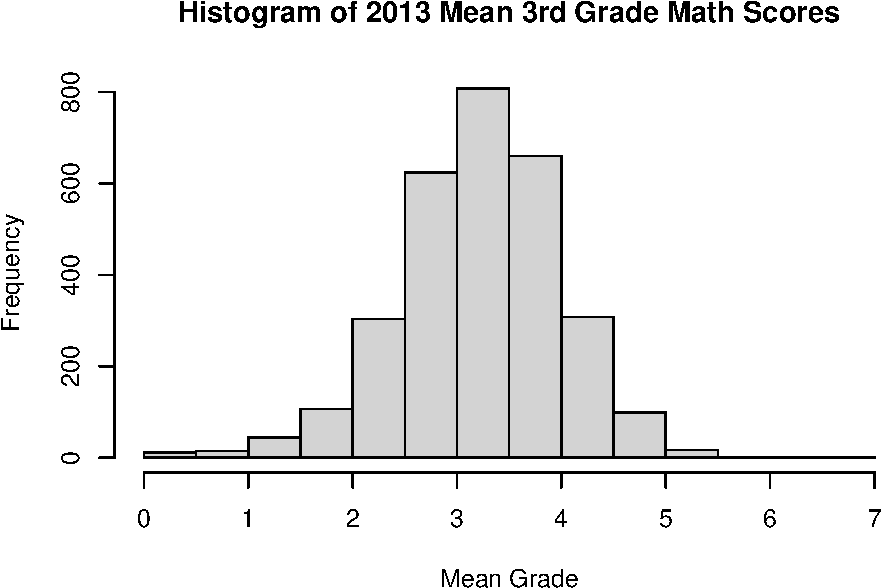
\includegraphics[keepaspectratio]{finalPaper_files/figure-latex/math-1.pdf}}

\subsection{Poverty Rate and Turnout
Rate}\label{poverty-rate-and-turnout-rate}

To see the relationship between voter turnout and one predictor variable
hypothesized to be associated with it, we plot the 2010 poverty rate
against the 2020 turnout rate for each county. There is a strong
negative trend in the plot.

\begin{Shaded}
\begin{Highlighting}[]
\FunctionTok{plot}\NormalTok{(turnout\_data}\SpecialCharTok{$}\NormalTok{poor\_share2010, turnout\_data}\SpecialCharTok{$}\NormalTok{turnout.rate, }\AttributeTok{main =} \StringTok{\textquotesingle{}Turnout Rate vs. Poverty Rate\textquotesingle{}}\NormalTok{, }\AttributeTok{xlab =} \StringTok{\textquotesingle{}2010 Poverty Rate\textquotesingle{}}\NormalTok{, }\AttributeTok{ylab =} \StringTok{\textquotesingle{}2020 Turnout Rate\textquotesingle{}}\NormalTok{)}
\end{Highlighting}
\end{Shaded}

\pandocbounded{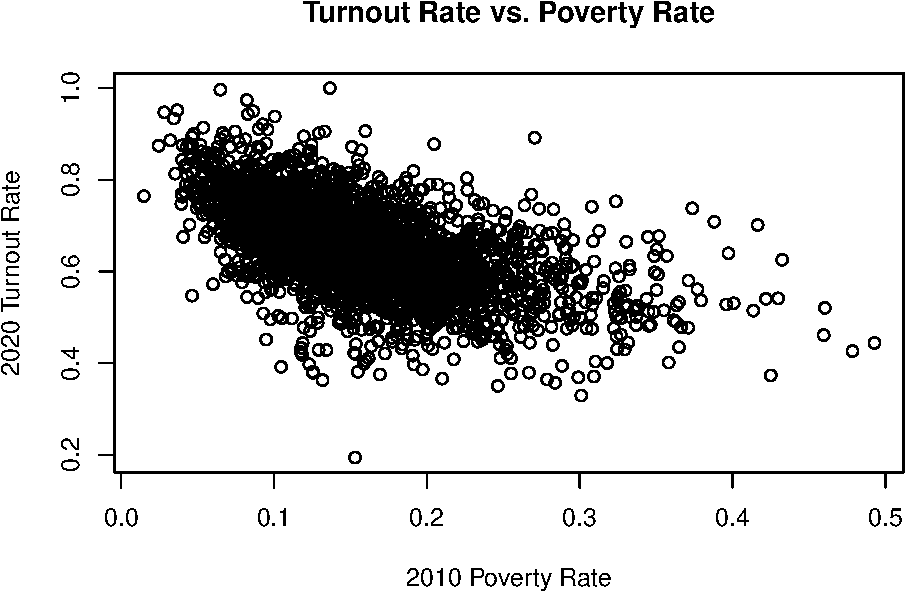
\includegraphics[keepaspectratio]{finalPaper_files/figure-latex/poverty-1.pdf}}

\section{Preliminary Model}\label{preliminary-model}

We also check that our hypothesis that the turnout rate can be predicted
from county demographics is reasonable by fitting a linear regression
model.

\begin{Shaded}
\begin{Highlighting}[]
\NormalTok{lm\_model }\OtherTok{\textless{}{-}} \FunctionTok{lm}\NormalTok{(turnout.rate }\SpecialCharTok{\textasciitilde{}}\NormalTok{ . }\SpecialCharTok{{-}}\NormalTok{ (State }\SpecialCharTok{+}\NormalTok{ County }\SpecialCharTok{+}\NormalTok{ fips), }\AttributeTok{data =}\NormalTok{ turnout\_data)}
\FunctionTok{summary}\NormalTok{(lm\_model)}
\end{Highlighting}
\end{Shaded}

\begin{verbatim}
## 
## Call:
## lm(formula = turnout.rate ~ . - (State + County + fips), data = turnout_data)
## 
## Residuals:
##      Min       1Q   Median       3Q      Max 
## -0.47572 -0.04720 -0.00065  0.04700  0.30720 
## 
## Coefficients:
##                                Estimate Std. Error t value Pr(>|t|)    
## (Intercept)                   6.083e-01  3.290e-02  18.489  < 2e-16 ***
## frac_coll_plus2010            3.718e-01  2.598e-02  14.313  < 2e-16 ***
## foreign_share2010             1.105e-01  4.960e-02   2.227 0.026033 *  
## med_hhinc2016                 1.296e-07  2.543e-07   0.510 0.610193    
## poor_share2010               -5.756e-01  4.036e-02 -14.262  < 2e-16 ***
## share_white2010               4.233e-02  2.082e-02   2.033 0.042122 *  
## share_black2010               5.908e-02  2.084e-02   2.835 0.004615 ** 
## share_hisp2010               -5.112e-02  2.486e-02  -2.056 0.039840 *  
## share_asian2010              -5.062e-01  9.173e-02  -5.519 3.71e-08 ***
## gsmn_math_g3_2013            -9.931e-04  2.142e-03  -0.464 0.642954    
## rent_twobed2015              -7.016e-06  1.425e-05  -0.492 0.622587    
## singleparent_share2010       -6.174e-02  2.455e-02  -2.515 0.011971 *  
## traveltime15_2010            -4.253e-02  1.170e-02  -3.634 0.000283 ***
## emp2000                       1.137e-01  2.729e-02   4.167 3.17e-05 ***
## popdensity2010               -2.256e-07  5.510e-06  -0.041 0.967336    
## ann_avg_job_growth_2004_2013 -7.074e-01  1.068e-01  -6.624 4.12e-11 ***
## job_density_2013             -4.916e-06  1.134e-05  -0.434 0.664669    
## ---
## Signif. codes:  0 '***' 0.001 '**' 0.01 '*' 0.05 '.' 0.1 ' ' 1
## 
## Residual standard error: 0.07304 on 2982 degrees of freedom
## Multiple R-squared:  0.4416, Adjusted R-squared:  0.4386 
## F-statistic: 147.4 on 16 and 2982 DF,  p-value: < 2.2e-16
\end{verbatim}

The linear regression model examining voter turnout demonstrates several
significant relationships while controlling for State, County, and FIPS
fixed effects. The model explains approximately 44\% of the variance in
turnout rates (Adjusted R-squared = \(0.4386\)) and is highly
significant (F = \(147.4\), \(p < 2.2 \times 10^{-16}\)). Education
emerges as a strong positive predictor, with a one-unit increase in
college education associated with a \(0.371\) increase in turnout
(\(p < 0.001\)). Other significant positive predictors include
foreign-born share (\(\beta = 0.110\), \(p < 0.05\)), white population
share (\(\beta = 0.042\), \(p < 0.05\)), black population share
(\(\beta = 0.059\), \(p < 0.01\)), and employment (\(\beta = 0.137\),
\(p < 0.001\)). Conversely, several factors show significant negative
associations with turnout: poverty rate exhibits a strong negative
effect (\(\beta = -0.576\), \(p < 0.001\)), as do Asian population share
(\(\beta = -0.506\), \(p < 0.001\)), single parent share
(\(\beta = -0.062\), \(p < 0.05\)), travel time (\(\beta = -0.043\),
\(p < 0.001\)), and job growth (\(\beta = -0.707\), \(p < 0.001\)).
Notably, several variables including median household income, Hispanic
population share, math scores, two-bedroom rent, population density, and
job density did not show significant relationships with turnout
(\(p > 0.05\)). The residual standard error of \(0.073\) on \(2982\)
degrees of freedom suggests relatively precise estimates, while the
overall model significance (\(p < 2.2 \times 10^{-16}\)) indicates
strong explanatory power in predicting voter turnout rates.

\section{Diagnostics}\label{diagnostics}

\begin{Shaded}
\begin{Highlighting}[]
\FunctionTok{plot}\NormalTok{(lm\_model, }\FunctionTok{c}\NormalTok{(}\DecValTok{1}\NormalTok{, }\DecValTok{2}\NormalTok{))}
\end{Highlighting}
\end{Shaded}

\pandocbounded{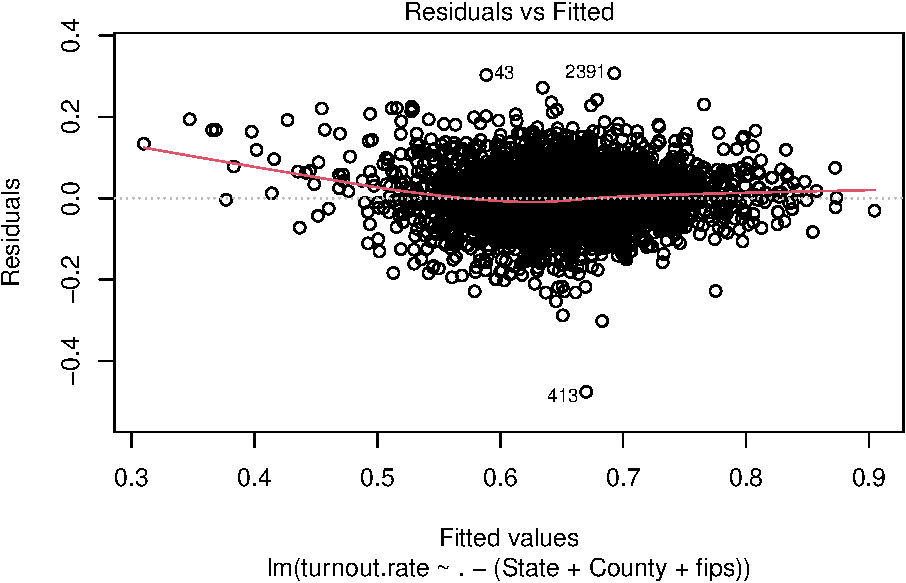
\includegraphics[keepaspectratio]{finalPaper_files/figure-latex/diagnostics-1.pdf}}
\pandocbounded{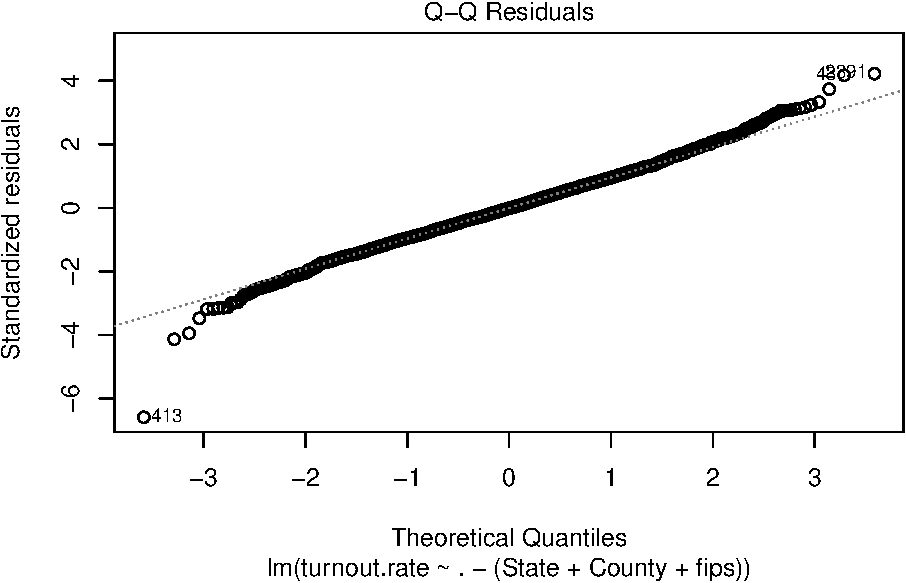
\includegraphics[keepaspectratio]{finalPaper_files/figure-latex/diagnostics-2.pdf}}

\subsection{Existence of Variance}\label{existence-of-variance}

The spread of residuals in the plots demonstrates clear variation in our
dependent variable, confirming the existence of variance. The residuals
show a reasonable spread around zero, with most falling between -0.2 and
0.2, indicating that our model has captured meaningful variation in the
data while maintaining reasonable error terms.

\subsection{Linearity}\label{linearity}

The Residuals vs Fitted plot reveals a relatively flat red line hovering
around zero, suggesting the linearity assumption is reasonably met.
While there is some pattern in the spread of residuals, the scatter
appears generally random. The plot identifies points 43, 2391, and 413
as potential outliers that warrant further investigation. Overall, the
linearity assumption appears to be satisfied, though with some potential
concerns that might need additional examination.

\subsection{Independence}\label{independence}

Independence cannot be directly assessed from these diagnostic plots
alone. Given that this analysis uses county-level data, there is likely
spatial correlation present between neighboring counties. Additional
specific tests would be necessary to evaluate this assumption, such as
Moran's I for spatial autocorrelation. We hope to ask a Teaching Fellow
about further analysis regarding this possible violation of our
assumptions.

\subsection{Homogeneity
(Homoscedasticity)}\label{homogeneity-homoscedasticity}

Examining the Residuals vs Fitted plot, we observe a fanning pattern
where the spread of residuals is wider in the middle range of fitted
values. This pattern suggests the presence of heteroscedasticity,
meaning the variance of residuals is not constant across all fitted
values. This violation of the homoscedasticity assumption suggests we
should consider using robust standard errors or weighted least squares
estimation methods to address this issue.

\subsection{Normality}\label{normality}

The Q-Q plot provides a visual assessment of normality by comparing the
standardized residuals against theoretical normal quantiles. The
majority of points follow the diagonal line, suggesting approximate
normality in the central region of the distribution. However, we observe
some deviation at both tails, particularly with point 413 showing as a
significant lower outlier and points near 43 \& 2391 deviating at the
upper tail. Given our large sample size, the Central Limit Theorem
suggests that these deviations from normality are less concerning for
inference purposes.

\section{Overall Recommendations and Next
Steps}\label{overall-recommendations-and-next-steps}

Based on these diagnostics, several actions are recommended. First,
investigate points 413, 43, and 2391 for potential data issues or
substantive influence. Second, implement robust standard errors to
address the observed possible heteroscedasticity. Third, consider
spatial correlation adjustments given the county-level nature of the
data.

Regarding the model, we will test interaction terms to see how different
factors affect each other. We will also observe how applying
regularization impacts our regression.

\begin{Shaded}
\begin{Highlighting}[]
\FunctionTok{library}\NormalTok{(glmnet)}
\FunctionTok{library}\NormalTok{(pheatmap)}

\NormalTok{predictors }\OtherTok{\textless{}{-}} \FunctionTok{names}\NormalTok{(turnout\_data)[}\SpecialCharTok{!}\NormalTok{(}\FunctionTok{names}\NormalTok{(turnout\_data) }\SpecialCharTok{\%in\%} \FunctionTok{c}\NormalTok{(}\StringTok{\textquotesingle{}State\textquotesingle{}}\NormalTok{, }\StringTok{\textquotesingle{}County\textquotesingle{}}\NormalTok{, }\StringTok{\textquotesingle{}fips\textquotesingle{}}\NormalTok{, }\StringTok{\textquotesingle{}turnout.rate\textquotesingle{}}\NormalTok{))]}
\NormalTok{x }\OtherTok{\textless{}{-}} \FunctionTok{model.matrix}\NormalTok{(turnout.rate }\SpecialCharTok{\textasciitilde{}}\NormalTok{ . }\SpecialCharTok{{-}}\NormalTok{ (State }\SpecialCharTok{+}\NormalTok{ County }\SpecialCharTok{+}\NormalTok{ fips), }\AttributeTok{data =}\NormalTok{ turnout\_data)[, }\SpecialCharTok{{-}}\DecValTok{1}\NormalTok{]}
\NormalTok{y }\OtherTok{\textless{}{-}}\NormalTok{ turnout\_data}\SpecialCharTok{$}\NormalTok{turnout.rate}

\FunctionTok{set.seed}\NormalTok{(}\DecValTok{82}\NormalTok{)}
\NormalTok{cv.lasso }\OtherTok{\textless{}{-}} \FunctionTok{cv.glmnet}\NormalTok{(x, y, }\AttributeTok{alpha =} \DecValTok{1}\NormalTok{, }\AttributeTok{nfolds =} \DecValTok{10}\NormalTok{)}

\NormalTok{best\_lambda }\OtherTok{\textless{}{-}}\NormalTok{ cv.lasso}\SpecialCharTok{$}\NormalTok{lambda.min}

\NormalTok{lasso\_model }\OtherTok{\textless{}{-}} \FunctionTok{glmnet}\NormalTok{(x, y, }\AttributeTok{alpha =} \DecValTok{1}\NormalTok{, }\AttributeTok{lambda =}\NormalTok{ best\_lambda)}
\FunctionTok{coef}\NormalTok{(lasso\_model)}
\end{Highlighting}
\end{Shaded}

\begin{verbatim}
## 17 x 1 sparse Matrix of class "dgCMatrix"
##                                         s0
## (Intercept)                   6.121987e-01
## frac_coll_plus2010            3.632965e-01
## foreign_share2010             7.023135e-02
## med_hhinc2016                 4.442856e-08
## poor_share2010               -5.736737e-01
## share_white2010               3.394170e-02
## share_black2010               4.990823e-02
## share_hisp2010               -4.857310e-02
## share_asian2010              -4.695689e-01
## gsmn_math_g3_2013             .           
## rent_twobed2015               .           
## singleparent_share2010       -6.054149e-02
## traveltime15_2010            -4.123835e-02
## emp2000                       1.160911e-01
## popdensity2010               -8.432251e-07
## ann_avg_job_growth_2004_2013 -6.699229e-01
## job_density_2013             -3.165965e-06
\end{verbatim}

\begin{Shaded}
\begin{Highlighting}[]
\NormalTok{cols }\OtherTok{\textless{}{-}} \FunctionTok{rainbow}\NormalTok{(}\FunctionTok{ncol}\NormalTok{(x))}

\FunctionTok{plot}\NormalTok{(cv.lasso}\SpecialCharTok{$}\NormalTok{glmnet.fit, }\AttributeTok{xvar=}\StringTok{"lambda"}\NormalTok{, }\AttributeTok{label=}\ConstantTok{TRUE}\NormalTok{, }\AttributeTok{col=}\NormalTok{cols, }\AttributeTok{lwd=}\DecValTok{2}\NormalTok{, }\AttributeTok{cex.lab=}\FloatTok{1.2}\NormalTok{, }\AttributeTok{cex.axis=}\FloatTok{1.2}\NormalTok{)}
\FunctionTok{abline}\NormalTok{(}\AttributeTok{v =} \FunctionTok{log}\NormalTok{(best\_lambda), }\AttributeTok{lty=}\DecValTok{2}\NormalTok{, }\AttributeTok{col=}\StringTok{"red"}\NormalTok{, }\AttributeTok{lwd=}\DecValTok{2}\NormalTok{)}
\FunctionTok{title}\NormalTok{(}\StringTok{"LASSO Coefficients as Function of Regularization Strength"}\NormalTok{, }\AttributeTok{cex.main=}\FloatTok{1.2}\NormalTok{)}

\FunctionTok{legend}\NormalTok{(}\StringTok{"topright"}\NormalTok{, }\AttributeTok{inset=}\FunctionTok{c}\NormalTok{(}\SpecialCharTok{{-}}\FloatTok{0.1}\NormalTok{,}\DecValTok{0}\NormalTok{), }\AttributeTok{legend =} \FunctionTok{colnames}\NormalTok{(x), }\AttributeTok{col =}\NormalTok{ cols, }\AttributeTok{lty=}\DecValTok{1}\NormalTok{, }\AttributeTok{lwd=}\DecValTok{2}\NormalTok{, }\AttributeTok{cex=}\FloatTok{0.6}\NormalTok{, }\AttributeTok{xpd=}\ConstantTok{TRUE}\NormalTok{)}
\end{Highlighting}
\end{Shaded}

\pandocbounded{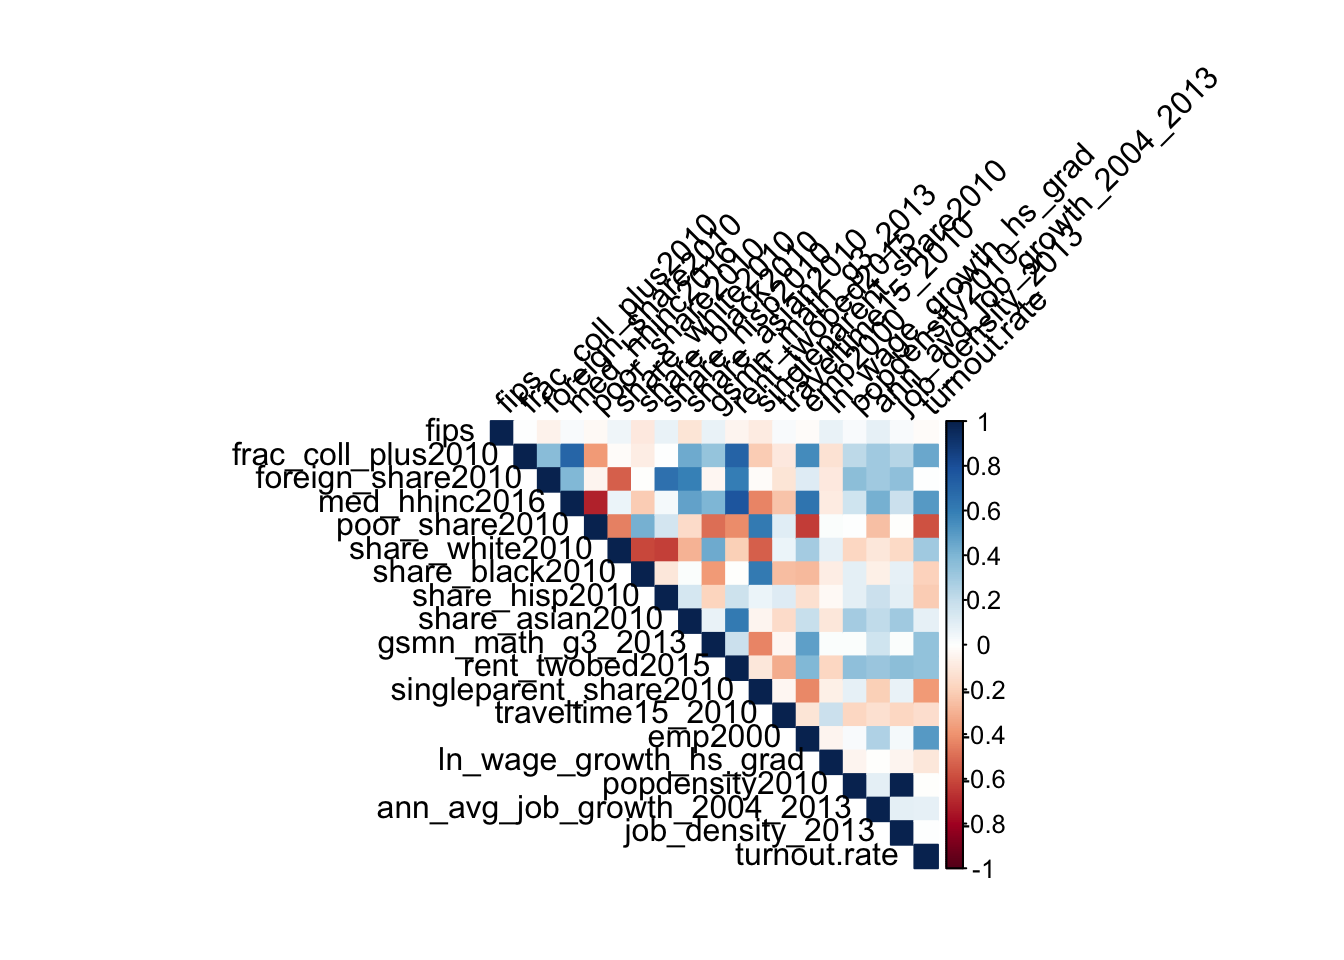
\includegraphics[keepaspectratio]{finalPaper_files/figure-latex/unnamed-chunk-4-1.pdf}}

\begin{Shaded}
\begin{Highlighting}[]
\NormalTok{coeffs }\OtherTok{\textless{}{-}} \FunctionTok{coef}\NormalTok{(lasso\_model)}

\NormalTok{coeffs\_df }\OtherTok{\textless{}{-}} \FunctionTok{as.data.frame}\NormalTok{(}\FunctionTok{as.matrix}\NormalTok{(coeffs))}
\FunctionTok{colnames}\NormalTok{(coeffs\_df) }\OtherTok{\textless{}{-}} \StringTok{"Coefficient"}
\NormalTok{coeffs\_df}\SpecialCharTok{$}\NormalTok{Predictor }\OtherTok{\textless{}{-}} \FunctionTok{rownames}\NormalTok{(coeffs\_df)}

\NormalTok{coeffs\_df }\OtherTok{\textless{}{-}} \FunctionTok{subset}\NormalTok{(coeffs\_df, Predictor }\SpecialCharTok{!=} \StringTok{"(Intercept)"}\NormalTok{)}

\NormalTok{kept }\OtherTok{\textless{}{-}}\NormalTok{ coeffs\_df}\SpecialCharTok{$}\NormalTok{Predictor[coeffs\_df}\SpecialCharTok{$}\NormalTok{Coefficient }\SpecialCharTok{!=} \DecValTok{0}\NormalTok{]}
\NormalTok{not\_kept }\OtherTok{\textless{}{-}}\NormalTok{ coeffs\_df}\SpecialCharTok{$}\NormalTok{Predictor[coeffs\_df}\SpecialCharTok{$}\NormalTok{Coefficient }\SpecialCharTok{==} \DecValTok{0}\NormalTok{]}

\FunctionTok{cat}\NormalTok{(}\StringTok{"Predictors kept by LASSO:}\SpecialCharTok{\textbackslash{}n}\StringTok{"}\NormalTok{)}
\end{Highlighting}
\end{Shaded}

\begin{verbatim}
## Predictors kept by LASSO:
\end{verbatim}

\begin{Shaded}
\begin{Highlighting}[]
\FunctionTok{print}\NormalTok{(kept)}
\end{Highlighting}
\end{Shaded}

\begin{verbatim}
##  [1] "frac_coll_plus2010"           "foreign_share2010"           
##  [3] "med_hhinc2016"                "poor_share2010"              
##  [5] "share_white2010"              "share_black2010"             
##  [7] "share_hisp2010"               "share_asian2010"             
##  [9] "singleparent_share2010"       "traveltime15_2010"           
## [11] "emp2000"                      "popdensity2010"              
## [13] "ann_avg_job_growth_2004_2013" "job_density_2013"
\end{verbatim}

\begin{Shaded}
\begin{Highlighting}[]
\FunctionTok{cat}\NormalTok{(}\StringTok{"}\SpecialCharTok{\textbackslash{}n}\StringTok{Predictors removed by LASSO (coefficients = 0):}\SpecialCharTok{\textbackslash{}n}\StringTok{"}\NormalTok{)}
\end{Highlighting}
\end{Shaded}

\begin{verbatim}
## 
## Predictors removed by LASSO (coefficients = 0):
\end{verbatim}

\begin{Shaded}
\begin{Highlighting}[]
\FunctionTok{print}\NormalTok{(not\_kept)}
\end{Highlighting}
\end{Shaded}

\begin{verbatim}
## [1] "gsmn_math_g3_2013" "rent_twobed2015"
\end{verbatim}

Running the LASSO regularization found an optimal lambda that zeroed out
the features gsmn\_math\_g3\_2013 as well as rent\_twobed2015. This
seems to align with our preliminary analysis that showed that both of
these predictors had p-values that were far above our p=0.05 threshold,
both at p\textgreater0.60.

\begin{Shaded}
\begin{Highlighting}[]
\NormalTok{cor\_matrix }\OtherTok{\textless{}{-}} \FunctionTok{cor}\NormalTok{(turnout\_data[, predictors], }\AttributeTok{use =} \StringTok{"pairwise.complete.obs"}\NormalTok{)}

\FunctionTok{pheatmap}\NormalTok{(cor\_matrix, }
  \AttributeTok{cluster\_rows =} \ConstantTok{TRUE}\NormalTok{, }
  \AttributeTok{cluster\_cols =} \ConstantTok{TRUE}\NormalTok{, }
  \AttributeTok{color =} \FunctionTok{colorRampPalette}\NormalTok{(}\FunctionTok{c}\NormalTok{(}\StringTok{"navy"}\NormalTok{, }\StringTok{"white"}\NormalTok{, }\StringTok{"firebrick3"}\NormalTok{))(}\DecValTok{50}\NormalTok{),}
  \AttributeTok{main =} \StringTok{"Heatmap of Predictor Correlations"}\NormalTok{,}
  \AttributeTok{height =} \DecValTok{50}\NormalTok{)  }
\end{Highlighting}
\end{Shaded}

\pandocbounded{\includegraphics[keepaspectratio]{finalPaper_files/figure-latex/unnamed-chunk-6-1.pdf}}

\begin{Shaded}
\begin{Highlighting}[]
\NormalTok{model\_reduced }\OtherTok{\textless{}{-}} \FunctionTok{lm}\NormalTok{(turnout.rate }\SpecialCharTok{\textasciitilde{}}\NormalTok{ . }\SpecialCharTok{{-}}\NormalTok{ State }\SpecialCharTok{{-}}\NormalTok{ County }\SpecialCharTok{{-}}\NormalTok{ fips }\SpecialCharTok{{-}}\NormalTok{ gsmn\_math\_g3\_2013 }\SpecialCharTok{{-}}\NormalTok{ rent\_twobed2015, }\AttributeTok{data =}\NormalTok{ turnout\_data)}

\NormalTok{model\_full }\OtherTok{\textless{}{-}} \FunctionTok{lm}\NormalTok{(turnout.rate }\SpecialCharTok{\textasciitilde{}}\NormalTok{ . }\SpecialCharTok{{-}}\NormalTok{ State }\SpecialCharTok{{-}}\NormalTok{ County }\SpecialCharTok{{-}}\NormalTok{ fips }\SpecialCharTok{{-}}\NormalTok{ gsmn\_math\_g3\_2013 }\SpecialCharTok{{-}}\NormalTok{ rent\_twobed2015 }
                 \SpecialCharTok{+}\NormalTok{ frac\_coll\_plus2010}\SpecialCharTok{:}\NormalTok{poor\_share2010, }
                 \AttributeTok{data =}\NormalTok{ turnout\_data)}

\NormalTok{anova\_test }\OtherTok{\textless{}{-}} \FunctionTok{anova}\NormalTok{(model\_reduced, model\_full)}
\NormalTok{anova\_test}
\end{Highlighting}
\end{Shaded}

\begin{verbatim}
## Analysis of Variance Table
## 
## Model 1: turnout.rate ~ (State + County + fips + frac_coll_plus2010 + 
##     foreign_share2010 + med_hhinc2016 + poor_share2010 + share_white2010 + 
##     share_black2010 + share_hisp2010 + share_asian2010 + gsmn_math_g3_2013 + 
##     rent_twobed2015 + singleparent_share2010 + traveltime15_2010 + 
##     emp2000 + popdensity2010 + ann_avg_job_growth_2004_2013 + 
##     job_density_2013) - State - County - fips - gsmn_math_g3_2013 - 
##     rent_twobed2015
## Model 2: turnout.rate ~ (State + County + fips + frac_coll_plus2010 + 
##     foreign_share2010 + med_hhinc2016 + poor_share2010 + share_white2010 + 
##     share_black2010 + share_hisp2010 + share_asian2010 + gsmn_math_g3_2013 + 
##     rent_twobed2015 + singleparent_share2010 + traveltime15_2010 + 
##     emp2000 + popdensity2010 + ann_avg_job_growth_2004_2013 + 
##     job_density_2013) - State - County - fips - gsmn_math_g3_2013 - 
##     rent_twobed2015 + frac_coll_plus2010:poor_share2010
##   Res.Df   RSS Df Sum of Sq      F    Pr(>F)    
## 1   2984 15.91                                  
## 2   2983 15.42  1   0.49052 94.894 < 2.2e-16 ***
## ---
## Signif. codes:  0 '***' 0.001 '**' 0.01 '*' 0.05 '.' 0.1 ' ' 1
\end{verbatim}

P value 2.2e-16 signifcant.. means that interaction term is significant
and helps to explain the variance in the model.

\begin{Shaded}
\begin{Highlighting}[]
\NormalTok{model\_post\_lasso }\OtherTok{\textless{}{-}} \FunctionTok{lm}\NormalTok{(}
\NormalTok{  turnout.rate }\SpecialCharTok{\textasciitilde{}}\NormalTok{ . }\SpecialCharTok{{-}}\NormalTok{ State }\SpecialCharTok{{-}}\NormalTok{ County }\SpecialCharTok{{-}}\NormalTok{ fips }\SpecialCharTok{{-}}\NormalTok{ gsmn\_math\_g3\_2013 }\SpecialCharTok{{-}}\NormalTok{ rent\_twobed2015 }\SpecialCharTok{+} \FunctionTok{factor}\NormalTok{(State),}
  \AttributeTok{data =}\NormalTok{ turnout\_data}
\NormalTok{)}

\FunctionTok{summary}\NormalTok{(model\_post\_lasso)}
\end{Highlighting}
\end{Shaded}

\begin{verbatim}
## 
## Call:
## lm(formula = turnout.rate ~ . - State - County - fips - gsmn_math_g3_2013 - 
##     rent_twobed2015 + factor(State), data = turnout_data)
## 
## Residuals:
##      Min       1Q   Median       3Q      Max 
## -0.42729 -0.03049 -0.00122  0.03066  0.29353 
## 
## Coefficients:
##                                     Estimate Std. Error t value Pr(>|t|)    
## (Intercept)                        5.336e-01  2.979e-02  17.912  < 2e-16 ***
## frac_coll_plus2010                 2.398e-01  2.109e-02  11.373  < 2e-16 ***
## foreign_share2010                 -5.603e-02  4.458e-02  -1.257 0.208914    
## med_hhinc2016                      9.682e-07  2.088e-07   4.636 3.70e-06 ***
## poor_share2010                    -3.474e-01  3.486e-02  -9.966  < 2e-16 ***
## share_white2010                    9.735e-02  1.979e-02   4.918 9.21e-07 ***
## share_black2010                    1.042e-01  2.123e-02   4.908 9.73e-07 ***
## share_hisp2010                     3.103e-03  2.489e-02   0.125 0.900789    
## share_asian2010                   -5.204e-01  9.504e-02  -5.476 4.72e-08 ***
## singleparent_share2010            -8.936e-02  2.048e-02  -4.363 1.32e-05 ***
## traveltime15_2010                 -9.101e-02  1.159e-02  -7.851 5.76e-15 ***
## emp2000                            1.104e-01  2.520e-02   4.382 1.22e-05 ***
## popdensity2010                     5.026e-06  4.507e-06   1.115 0.264946    
## ann_avg_job_growth_2004_2013      -6.982e-01  9.184e-02  -7.603 3.88e-14 ***
## job_density_2013                  -1.071e-05  9.239e-06  -1.159 0.246589    
## factor(State)Alaska                1.608e-02  1.842e-02   0.873 0.382787    
## factor(State)Arizona               5.215e-02  1.747e-02   2.985 0.002861 ** 
## factor(State)Arkansas             -9.944e-02  9.917e-03 -10.027  < 2e-16 ***
## factor(State)California            4.921e-02  1.212e-02   4.062 5.00e-05 ***
## factor(State)Colorado              8.884e-02  1.148e-02   7.740 1.36e-14 ***
## factor(State)Connecticut          -4.244e-02  2.227e-02  -1.905 0.056830 .  
## factor(State)Delaware              2.913e-03  3.433e-02   0.085 0.932388    
## factor(State)District of Columbia -4.882e-02  5.958e-02  -0.819 0.412677    
## factor(State)Florida               4.820e-02  1.050e-02   4.591 4.61e-06 ***
## factor(State)Georgia              -1.941e-02  8.546e-03  -2.271 0.023205 *  
## factor(State)Hawaii                1.088e-01  3.992e-02   2.726 0.006444 ** 
## factor(State)Idaho                 4.300e-02  1.206e-02   3.566 0.000368 ***
## factor(State)Illinois             -2.579e-02  9.701e-03  -2.658 0.007893 ** 
## factor(State)Indiana              -7.224e-02  9.951e-03  -7.259 4.97e-13 ***
## factor(State)Iowa                  3.768e-02  1.008e-02   3.738 0.000189 ***
## factor(State)Kansas               -1.577e-02  1.011e-02  -1.560 0.118888    
## factor(State)Kentucky             -1.587e-02  9.438e-03  -1.682 0.092771 .  
## factor(State)Louisiana             1.088e-03  1.026e-02   0.106 0.915566    
## factor(State)Maine                 7.530e-02  1.659e-02   4.539 5.89e-06 ***
## factor(State)Maryland             -4.177e-02  1.432e-02  -2.918 0.003554 ** 
## factor(State)Massachusetts         2.107e-02  1.785e-02   1.181 0.237859    
## factor(State)Michigan              5.593e-02  1.006e-02   5.561 2.93e-08 ***
## factor(State)Minnesota             6.894e-02  1.032e-02   6.682 2.81e-11 ***
## factor(State)Mississippi           1.263e-03  9.723e-03   0.130 0.896657    
## factor(State)Missouri             -3.106e-02  9.426e-03  -3.295 0.000997 ***
## factor(State)Montana               7.623e-02  1.243e-02   6.133 9.75e-10 ***
## factor(State)Nebraska              2.503e-02  1.080e-02   2.318 0.020507 *  
## factor(State)Nevada                5.369e-02  1.873e-02   2.866 0.004183 ** 
## factor(State)New Hampshire         6.395e-03  2.012e-02   0.318 0.750609    
## factor(State)New Jersey            2.675e-02  1.563e-02   1.711 0.087174 .  
## factor(State)New Mexico            2.117e-02  1.497e-02   1.414 0.157338    
## factor(State)New York             -5.491e-02  1.112e-02  -4.939 8.30e-07 ***
## factor(State)North Carolina        4.468e-02  9.253e-03   4.829 1.44e-06 ***
## factor(State)North Dakota         -1.759e-03  1.251e-02  -0.141 0.888178    
## factor(State)Ohio                 -2.654e-02  9.949e-03  -2.668 0.007670 ** 
## factor(State)Oklahoma             -8.357e-02  1.053e-02  -7.934 2.99e-15 ***
## factor(State)Oregon                1.182e-01  1.286e-02   9.191  < 2e-16 ***
## factor(State)Pennsylvania         -1.508e-02  1.052e-02  -1.433 0.152074    
## factor(State)Rhode Island         -5.543e-02  2.740e-02  -2.023 0.043192 *  
## factor(State)South Carolina        9.969e-04  1.132e-02   0.088 0.929836    
## factor(State)South Dakota          3.214e-03  1.180e-02   0.273 0.785250    
## factor(State)Tennessee            -6.913e-02  9.586e-03  -7.211 7.02e-13 ***
## factor(State)Texas                -2.023e-02  9.300e-03  -2.175 0.029692 *  
## factor(State)Utah                  4.048e-02  1.402e-02   2.888 0.003910 ** 
## factor(State)Vermont               3.112e-02  1.812e-02   1.718 0.085953 .  
## factor(State)Virginia              6.502e-03  8.997e-03   0.723 0.469910    
## factor(State)Washington            1.113e-01  1.247e-02   8.924  < 2e-16 ***
## factor(State)West Virginia        -8.496e-02  1.108e-02  -7.668 2.35e-14 ***
## factor(State)Wisconsin             5.134e-02  1.060e-02   4.841 1.36e-06 ***
## factor(State)Wyoming              -9.239e-03  1.497e-02  -0.617 0.537151    
## ---
## Signif. codes:  0 '***' 0.001 '**' 0.01 '*' 0.05 '.' 0.1 ' ' 1
## 
## Residual standard error: 0.058 on 2934 degrees of freedom
## Multiple R-squared:  0.6536, Adjusted R-squared:  0.646 
## F-statistic: 86.49 on 64 and 2934 DF,  p-value: < 2.2e-16
\end{verbatim}

\end{document}
